
\subsection{Debiasing Conceptor}
\newcite{karve2019conceptor} introduced conceptor debiasing. Given a set of gendered words $V:=\{v_1,v_2,\dots,v_n\}$ and their embeddings $E$, gender bias can be mitigated by multiplying the debiasing conceptor matrix$\neg C= I-C$, where $C$ is the conceptor matrix that minimizes the objective
\begin{eqnarray}
||E-CE||^2_F+\alpha^{-2}||E||^2_F
\end{eqnarray}
where $\alpha$ is a parameter. $C$ has an analytical solution
\begin{eqnarray}
C=\frac{1}{d}EE^{T}(\frac{1}{d}EE^{T}+\alpha^{-2}I)^{-1}
\end{eqnarray}
Intuitively, C is a soft projection matrix on the linear subspace where embeddings have the maximum bias. 
Once C is computed a debiased version of embeddings $X \in R^{t \times d}$  can be obtained by matrix multiplication $X(I-C)$.

\subsection{Hard Debasing}
We will also compare with the hard debiasing method proposed
by \newcite{mu2018all}, which is originally a postprocessing
technique for improving word
representations. \newcite{karve2019conceptor} adopted it as a
method for debiasing. Hard debiasing relies upon
the assumption that the first principal component of the
embedding vectors is a meaningful gender direction. The first principal component of $E$ is the gender direction $q$.

\subsection{DensRay}
DensRay \cite{dufter2019analytical} is an analytical method for identifying the
embedding subspace of certain linguistic features. It
identifies the ``gender subspace'' using a set of gendered words
$V:=\{v_1,v_2,\dots,v_n\}$ and their embeddings $E \in
R^{n\times d}$. In contrast to the above approaches it uses a function $l$ for the gender attribute:
$l:V\to \{-1,1\}$;
e.g. $l(\mbox{father})=1$, $l(\mbox{sister})=-1$. The objective of DensRay
is to find an orthogonal matrix $Q\in R^{d\times d}$ such
that $EQ$ is  a gender subspace.

Let $L_{=}:=\{(v,w)\in V\times V|l(v)=l(w)\}$ and define
$L_{\neq}$ analogously.  The DensRay objective
in \eqref{densray1} is to maximize the distance of the word
pairs from the same gender group ($L_{=}$) and minimize the
distance of the word pairs from the different gender group
($L_{\neq}$).
\begin{eqnarray}
\max\limits_{q} 
\sum_{(v,w)\in L_{\neq}}\alpha_{\neq}||q^\intercal d_{vw}||^2_2
-\sum_{(v,w)\in L_{=}}\alpha_{=}||q^\intercal d_{vw}||^2_2
\eqlabel{densray1}
\end{eqnarray}
where we define $d_{vw}:=e_v-e_w$. The objective can be simplified to 
\begin{eqnarray}
\max \limits_{q} q^\intercal(
\sum_{(v,w)\in L_{\neq}}\alpha_{\neq}||d_{vw}d_{vw}^\intercal ||^2_2-\sum_{(v,w)\in L_{=}}\alpha_{=}||d_{vw}d_{vw}^\intercal ||^2_2)q=:\max\limits_{q} q^\intercal Aq
\eqlabel{eq:densray2}
\end{eqnarray}
As stated in \cite{dufter2019analytical} $q$ is simply the eigenvector of $A$ corresponding to the largest eigenvalue.
$\alpha_{\neq},\alpha_{=}\in [0,1]$ are hyperparameters to balance the different optimization terms. 

Let $V_{+}:=\{v\in V|l(v)=1\}$ with corresponding embedding $E_{+} \in R^{n_+\times d}$ and define$V_{-}, E_{-}$ analogously. Also let the cross-covariance matrix $K_{+-}=Cov(E_{+}^\intercal,E_{-}^\intercal)$, if $n_{+}=n_{-}=n/2$, then matrix $A$ in \eqref{eq:densray2} can be reformulated into matrix form
\begin{eqnarray}
A=\frac{n}{2}\{\alpha_{\neq}[(n-2)(K_{+-}+K_{+-}^\intercal)+(E_{+}-E_{-})(E_{+}-E_{-})^\intercal]-\alpha_{=}(n-2)(K_{++}+K_{--})\}
\eqlabel{eq:densray3}
\end{eqnarray}
\enote{sl}{from the first term we can see densray intend to maximize the correlation between different groups, and maximize the differences of embeddings from different groups; the second term, minimize the correlation in same the group.}
\subsection{Removing Gender Information}

Hard debiasing and DensRay yield a gender dimension $q \in R^d$. In a contextualized language model like BERT each layer yields a contextualized embedding matrix $X \in R^{t \times d}$ where $t$ is the length of the sentence. To debias representations we simply zero out the projected values on $q$ for each position, that is we set $X^{\text{debiased}}_i = X_i -  (X_i^\intercal q) q$ for each position $i$.


\subsection{Comparison of the Approaches}
\seclabel{artexample}
 \figref{fig:example} shows artificially created two dimensional embeddings. The lines show the gender directions identified by hard debiasing and DensRay. In this example
 the first principal component does not correlate with gender. DensRay is able to handle this as it explicitly uses the labels.
 
As Conceptor debiasing does not compute a single direction of gender, but always needs to apply the full conceptor matrix, it is not possible to depict the direction in the figure. 
We argue that DensRay is more interpretable than Conceptor. It allows for example to assign token level gender scores easily. In addition it affects language model performance less than Conceptor debiasing, as we show later.
\begin{figure}[h]
	\centering
	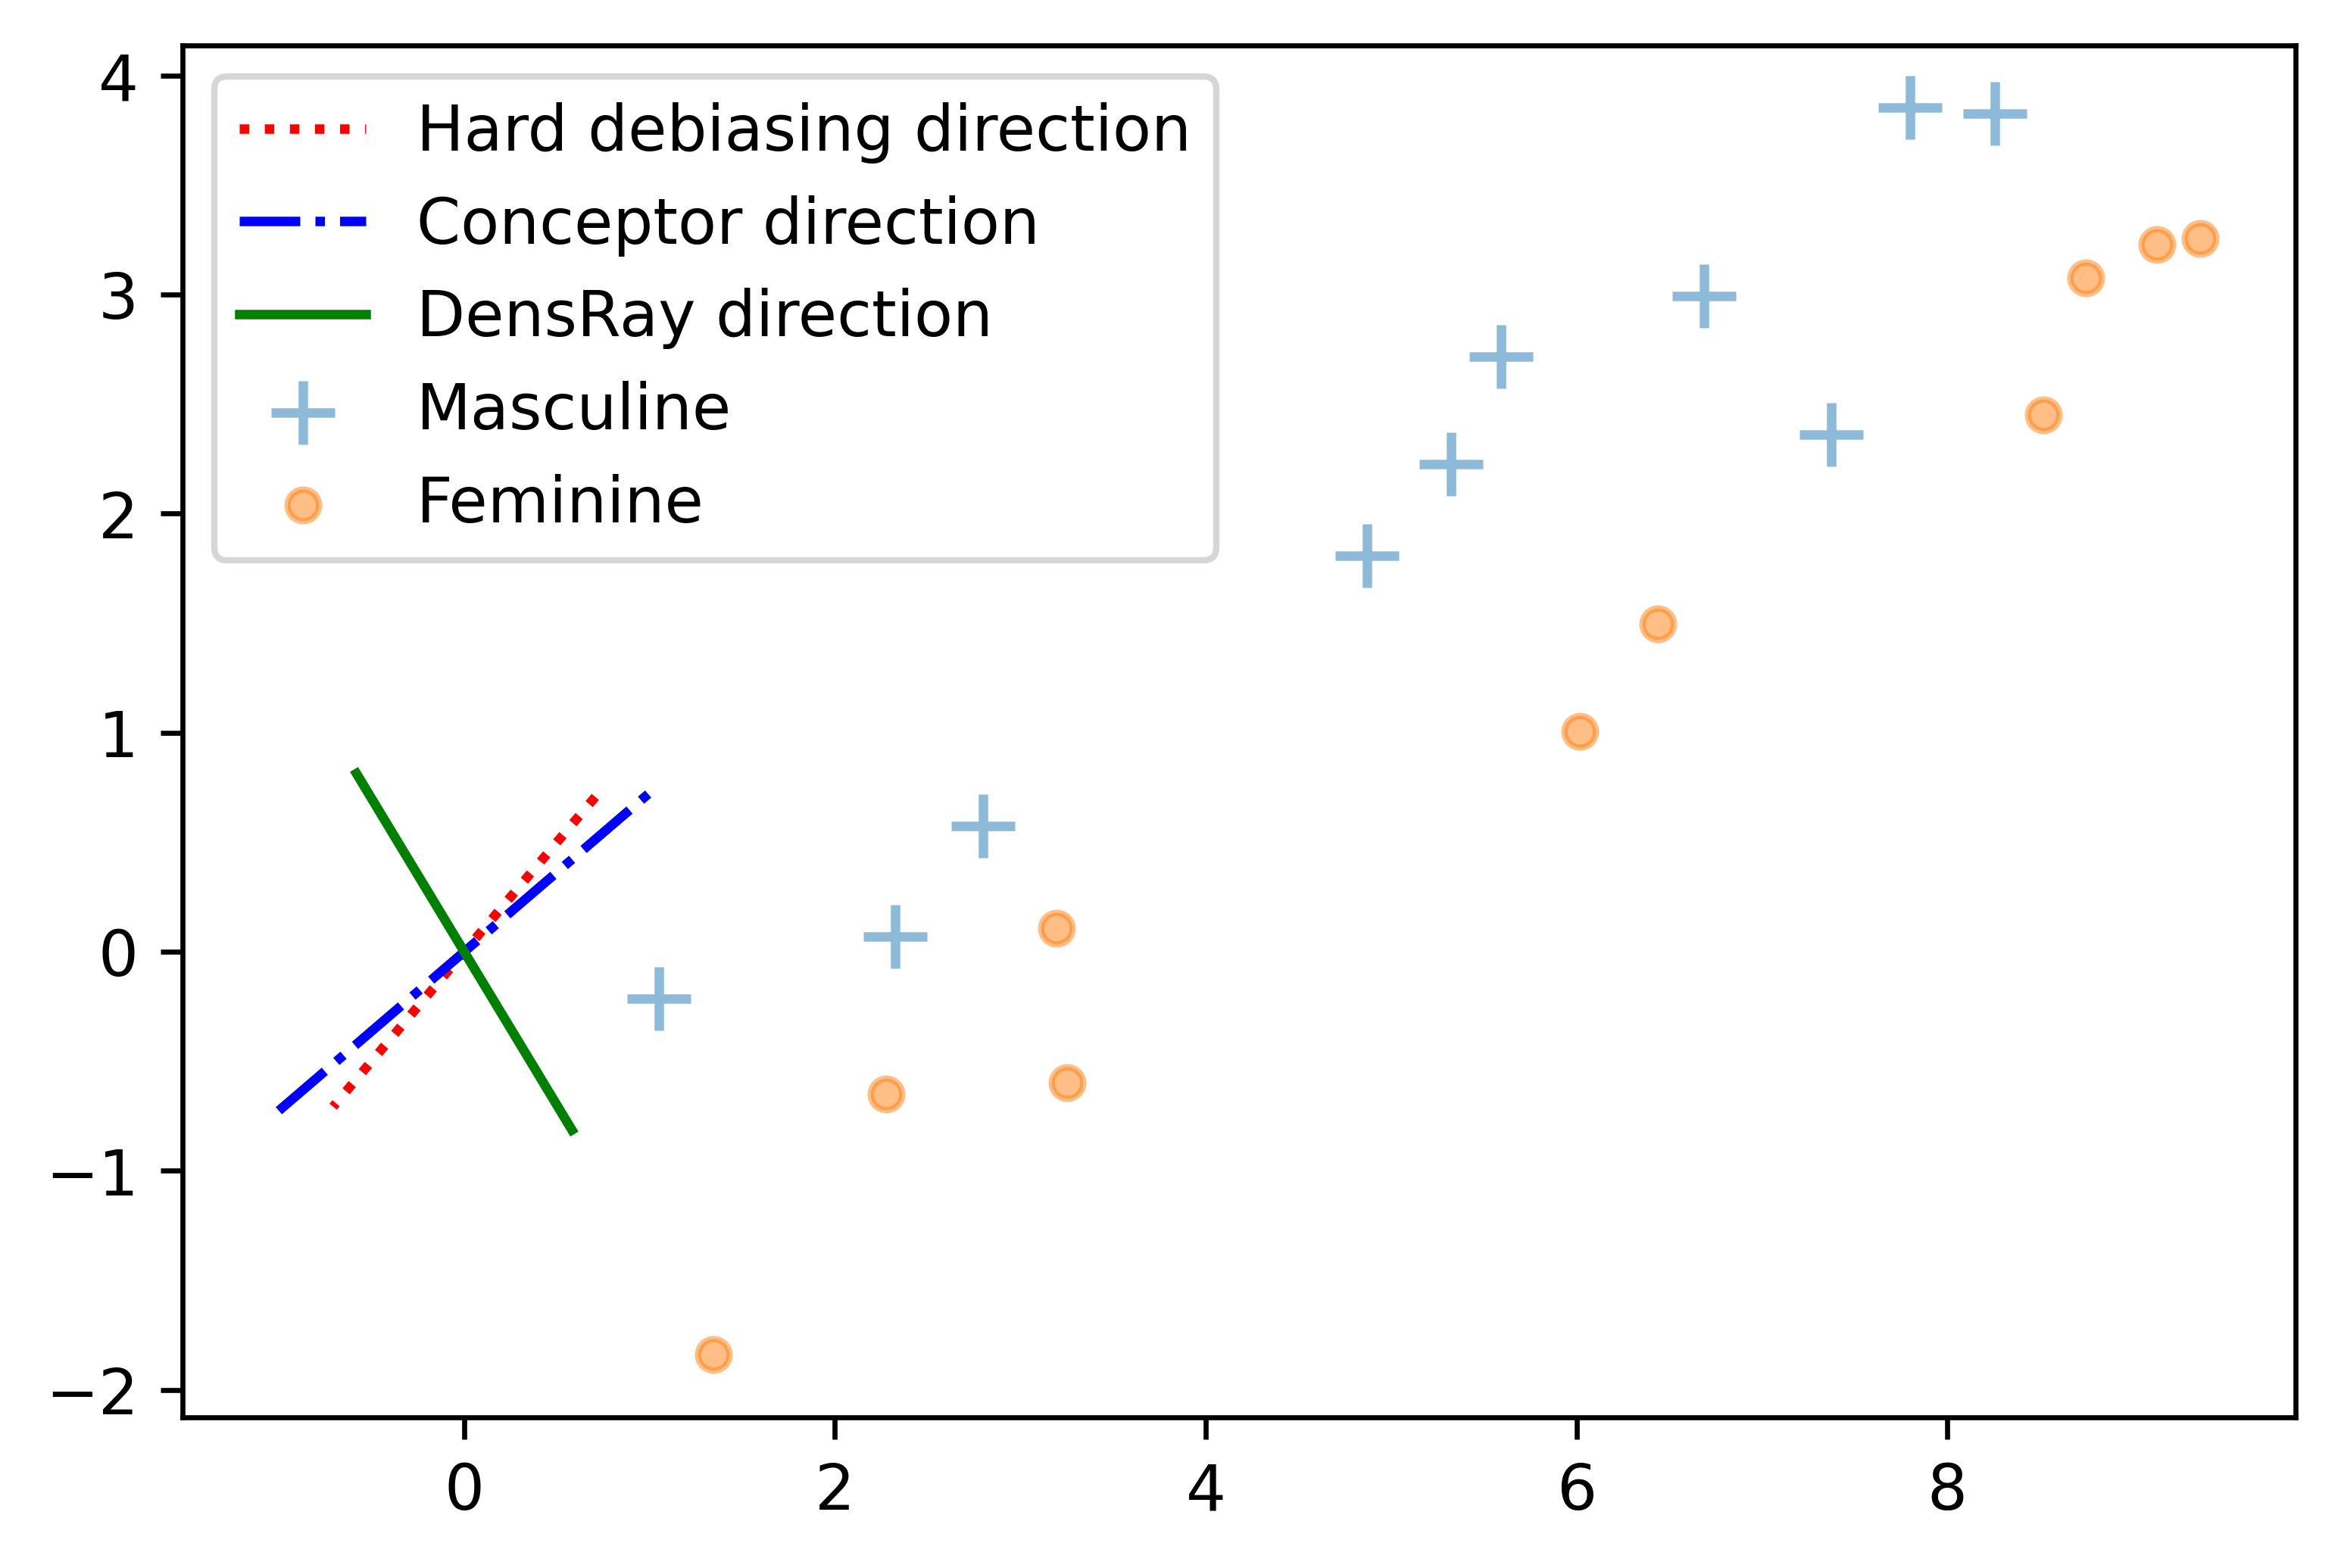
\includegraphics[width=0.4\linewidth]{examples.png}
	\caption{Gender direction for a set of gendered
          words computed for the three debiasing methods.}
	\figlabel{fig:example}
\end{figure}

\subsection{Adapting DensRay to Contextualized Language Models}
We now describe how we adapt DensRay to contextualized
language models. Given a set of gendered words
$V$, we extract sentences containing a word in $V$ from a
corpus. We run a contextualized language model
with $M$ layers
on a set of 
sentences that each contains one of the gender words, i.e., 
$t_1,\ldots,t_j,\ldots,t_n$ (where $t_j \in V$). 
For each $t_j $ in each sentence we  compute the contextualized representations $e_j^m, 1\leq m
\leq M$, one for each layer. We then use the vectors $e_j^m$ in \eqref{eq:densray2}.
to compute a gender direction
$q_m$ for the $m$th BERT layer. 
